\section{106 --- Construct Binary Tree from Inorder and Postorder Traversal}
Given inorder and postorder traversal of a tree, construct the binary tree.

\paragraph{Note:}
You may assume that duplicates do not exist in the tree.

For example, given

\fcj{inorder = [9,3,15,20,7]}

\fcj{postorder = [9,15,7,20,3]}

Return the following binary tree:

\begin{figure}[H]
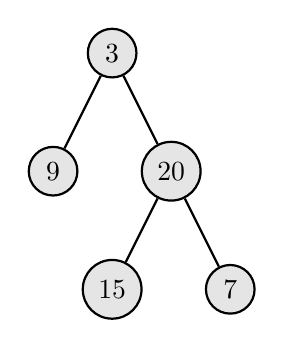
\begin{tikzpicture}
[every node/.style={draw, circle, fill=gray!20!, minimum size=5mm},
%level 1/.style={sibling distance=25mm},
%level 2/.style={sibling distance=15mm},
thick]
\node{3}
child{node{9}}
child{node{20} child{node{15}} child{node{7}}};
\end{tikzpicture}
\end{figure}
%\begin{figure}[H]
%\begin{tikzpicture}
%[mynode/.style={draw,circle,minimum size=10mm, fill=gray!20!}]
%\node(){};
%\node[mynode](3) {3};
%\node[mynode](9) [below = 8mm of 3, xshift=-10mm] {9};
%\node[mynode](20) [below = 8mm of 1, xshift=10mm] {20};
%\node[mynode](15) [below = 8mm of 20, xshift=-6mm] {15};
%\node[mynode](7) [below = 8mm of 20, xshift=6mm] {7};
%\draw[>=stealth,->] (3) -- (9);
%\draw[>=stealth,->] (3) -- (20);
%\draw[>=stealth,->] (20) -- (15);
%\draw[>=stealth,->] (20) -- (7);
%\end{tikzpicture}
%\end{figure}
\subsection{Recursion}
和105基本一样,唯一不同的是root是postorder数组的最后一个元素。递归函数其他部分都是一样的,即求出左子树长度和右子树长度,然后递归构建左子树和右子树。
%\setcounter{algorithm}{0}
%\begin{algorithm}[H]
%\caption{Recursion}
%\begin{algorithmic}[1]
%\Procedure{BuildTree}{$A, B, L$}
%\State $T:=\texttt{CreateTree}(A, 0, L, B, 0, L)$ \Comment Call \texttt{CreateTree} to create binary tree from $A[0,\ldots, L)$ and $B[0,\ldots,L)$
%\State \Return $T$
%\EndProcedure
%\end{algorithmic}
%\end{algorithm}
%\texttt{CreateTree}根据给定的\textbf{postorder}数组$A$和其范围$[p_0, p_1)$以及\textbf{inorder}数组$B$和其范围$[i_0, i_1)$构建出符合要求的binary tree
%\begin{algorithm}[H]
%\caption{Recursively Building Binary Tree}
%\begin{algorithmic}[1]
%\Function{CreateTree}{$A, p_0, p_1, B, i_0, i_1$}
%\If{$p_0\geq p_1$ \textbf{or} $i_0\geq i_1$} \Comment The ranges are not invalid
%\State \Return \texttt{null}
%\EndIf
%\State $\alpha:=i_0$
%\For{$i:=i_0$ \textbf{to} $i_1-1$}
%\If{$A[p_1-1]=B[i]$} \Comment The last element in $A$ is the root
%\State $\alpha\gets i$ \Comment Update the root position in $B$
%\State \texttt{break} \Comment Stop searching
%\EndIf
%\EndFor
%\State $L_0:=\alpha - i_0$ \Comment The left subtree length
%\State $L_1:=i_1 - \alpha - 1$ \Comment The right subtree length
%\State Create a new tree node $T$ with root value $A[i_0]$
%\State $\texttt{LEFT}(T)\gets \texttt{CreateTree}(A, p_0, p_0+L_0, B, i_0, \alpha)$ \Comment Create left subtree
%\State $\texttt{RIGHT}(T) \gets \texttt{CreateTree}(A, p_0+L_0, p_1-1, B, \alpha+1, i_1)$ \Comment Create right subtree
%\State \Return $T$
%\EndFunction
%\end{algorithmic}
%\end{algorithm}